%CHAPTER
\chapter{Návrh modulu}

%SECTION
\section{Vzhled PDF dokumentu}
\label{sec:navrh_vzhledu}
Při návrhu výsledného vzhledu celého dokumentu je potřeba klást důraz hlavně na co nejpřesnější vyobrazení webového formuláře do PDF souboru. Vzhled webového formuláře je zobrazen na obrázku \ref{fig:web_formular}.

%SUBSECTION
\subsection{Záhlaví}
Záhlaví dokumentu by mělo obsahovat jednoznačný identifikátor hodnotícího příspěvku doplněný o název vědeckého příspěvku, který bude hodnocen. Rozhodně by zde nemělo chybět ani logo konference TSD (ideálně ve vektorovém formátu). V případě, že název vědeckého příspěvku bude zasahovat do loga, tak bude zkráceno na fixní velikost.

%SUBSECTION
\subsection{Titulek}
Titulek dokumentu by měl uživateli jednoznačně říct, který vědecký příspěvek hodnotí (ideálně zobrazit název i identifikátor). V titulku by nemělo chybět ani jméno posuzovatele a doplňující informace ohledně vyplňování formuláře, případně ho informovat o nedostatcích a omezeních aktuálně vygenerovaného PDF dokumentu.

%SUBSECTION
\subsection{Formulář}
Vzhled formuláře by se měl v ideálním případě shodovat s webovým formulářem. První část formuláře obsahuje stupnicové hodnocení, zatímco druhá je spíše slovní formou. Po konzultaci s vedoucím práce bylo usouzeno, že element \textbf{Combo box} reprezentující stupnicové hodnocení parametru bude nahrazen skupinou elementů \textbf{Radio button}. Důvod tohoto rozhodnutí spočíval v lepším zobrazení hodnot na stupnici, doplněn o neschopnosti PHP generátorů zobrazit pěkný \textbf{Combo box} s bezproblémovou funkcionalitou (špatná manipulace při vybírání hodnot). Pro uložení doplňujícího textu byl použit element \textbf{Text area} pro případné poznámky ohledně stavu a obsahu vědeckého příspěvku. Element popisující \textit{Review state} a tlačítko \textit{Save review} nebudou do formuláře vloženy, jejich funkcionalita není potřebná pro modulem vytvářený formulář.

%SUBSECTION
\subsection{Hodnocený vědecký příspěvek}
Vygenerovaný dokument by měl hlavně sloužit pro vyplňování hodnotícího formuláře off-line a ideálně by měl obsahovat i veškerý obsah hodnoceného vědeckého příspěvku, aby měl posuzovatel možnost kdykoliv nahlédnout na jeho obsah. Tento příspěvek bude vložen na konec PDF souboru.

%SUBSECTION
\subsection{Vodoznak}
Ve světě se často stává, že se neoprávněně kopírují již hotová díla, která nejsou stále zaregistrovaná a mohou být případným zlodějem ukradnuta a vydána pod zlodějovo jménem. Proto je vhodné do celého dokumentu vložit vodoznak, který bude jasně říkat, že se jedná pouze o hodnotící soubor, nikoliv o plnohodnotné dílo.

%SUBSECTION
\subsection{Fonty}
\label{subsec:fonty}
V PDF a PostScript prostředí se lze setkat s pojmem \uv{14 standardních/základních fontů}. Tento pojem byl odvozen ze standardních 13 PostScript fontů a vyjadřuje základní fonty používané při vytváření veškerých PDF souborů. Všechny základní fonty lze nalézt v tabulce \ref{tab:table_basic_fonts}.

\begin{table}[h!]
\centering
\begin{tabular}{|l|l|} 
\hline
\textbf{Rodina fontů} & \textbf{Fonty}                                                                                               \\ 
\hline
\textit{Times}        & \begin{tabular}[c]{@{}l@{}}Times-Roman\\Times-Italic\\Times-Bold\\Times-BoldItalic\end{tabular}              \\ 
\hline
\textit{Helvetica}    & \begin{tabular}[c]{@{}l@{}}Helvetica\\Helvetica-Oblique\\Helvetica-Bold\\Helvetica-BoldOblique\end{tabular}  \\ 
\hline
\textit{Courier}      & \begin{tabular}[c]{@{}l@{}}Courier\\Courier-Oblique\\Courier-Bold\\Courier-BoldOblique\end{tabular}          \\ 
\hline
\textit{Symbol}       & Symbol                                                                                                       \\
\hline
\end{tabular}
\caption{Tabulka základních fontů pro PDF soubory%
\label{tab:table_basic_fonts}}
\end{table}

\begin{figure}[h!]
\centering
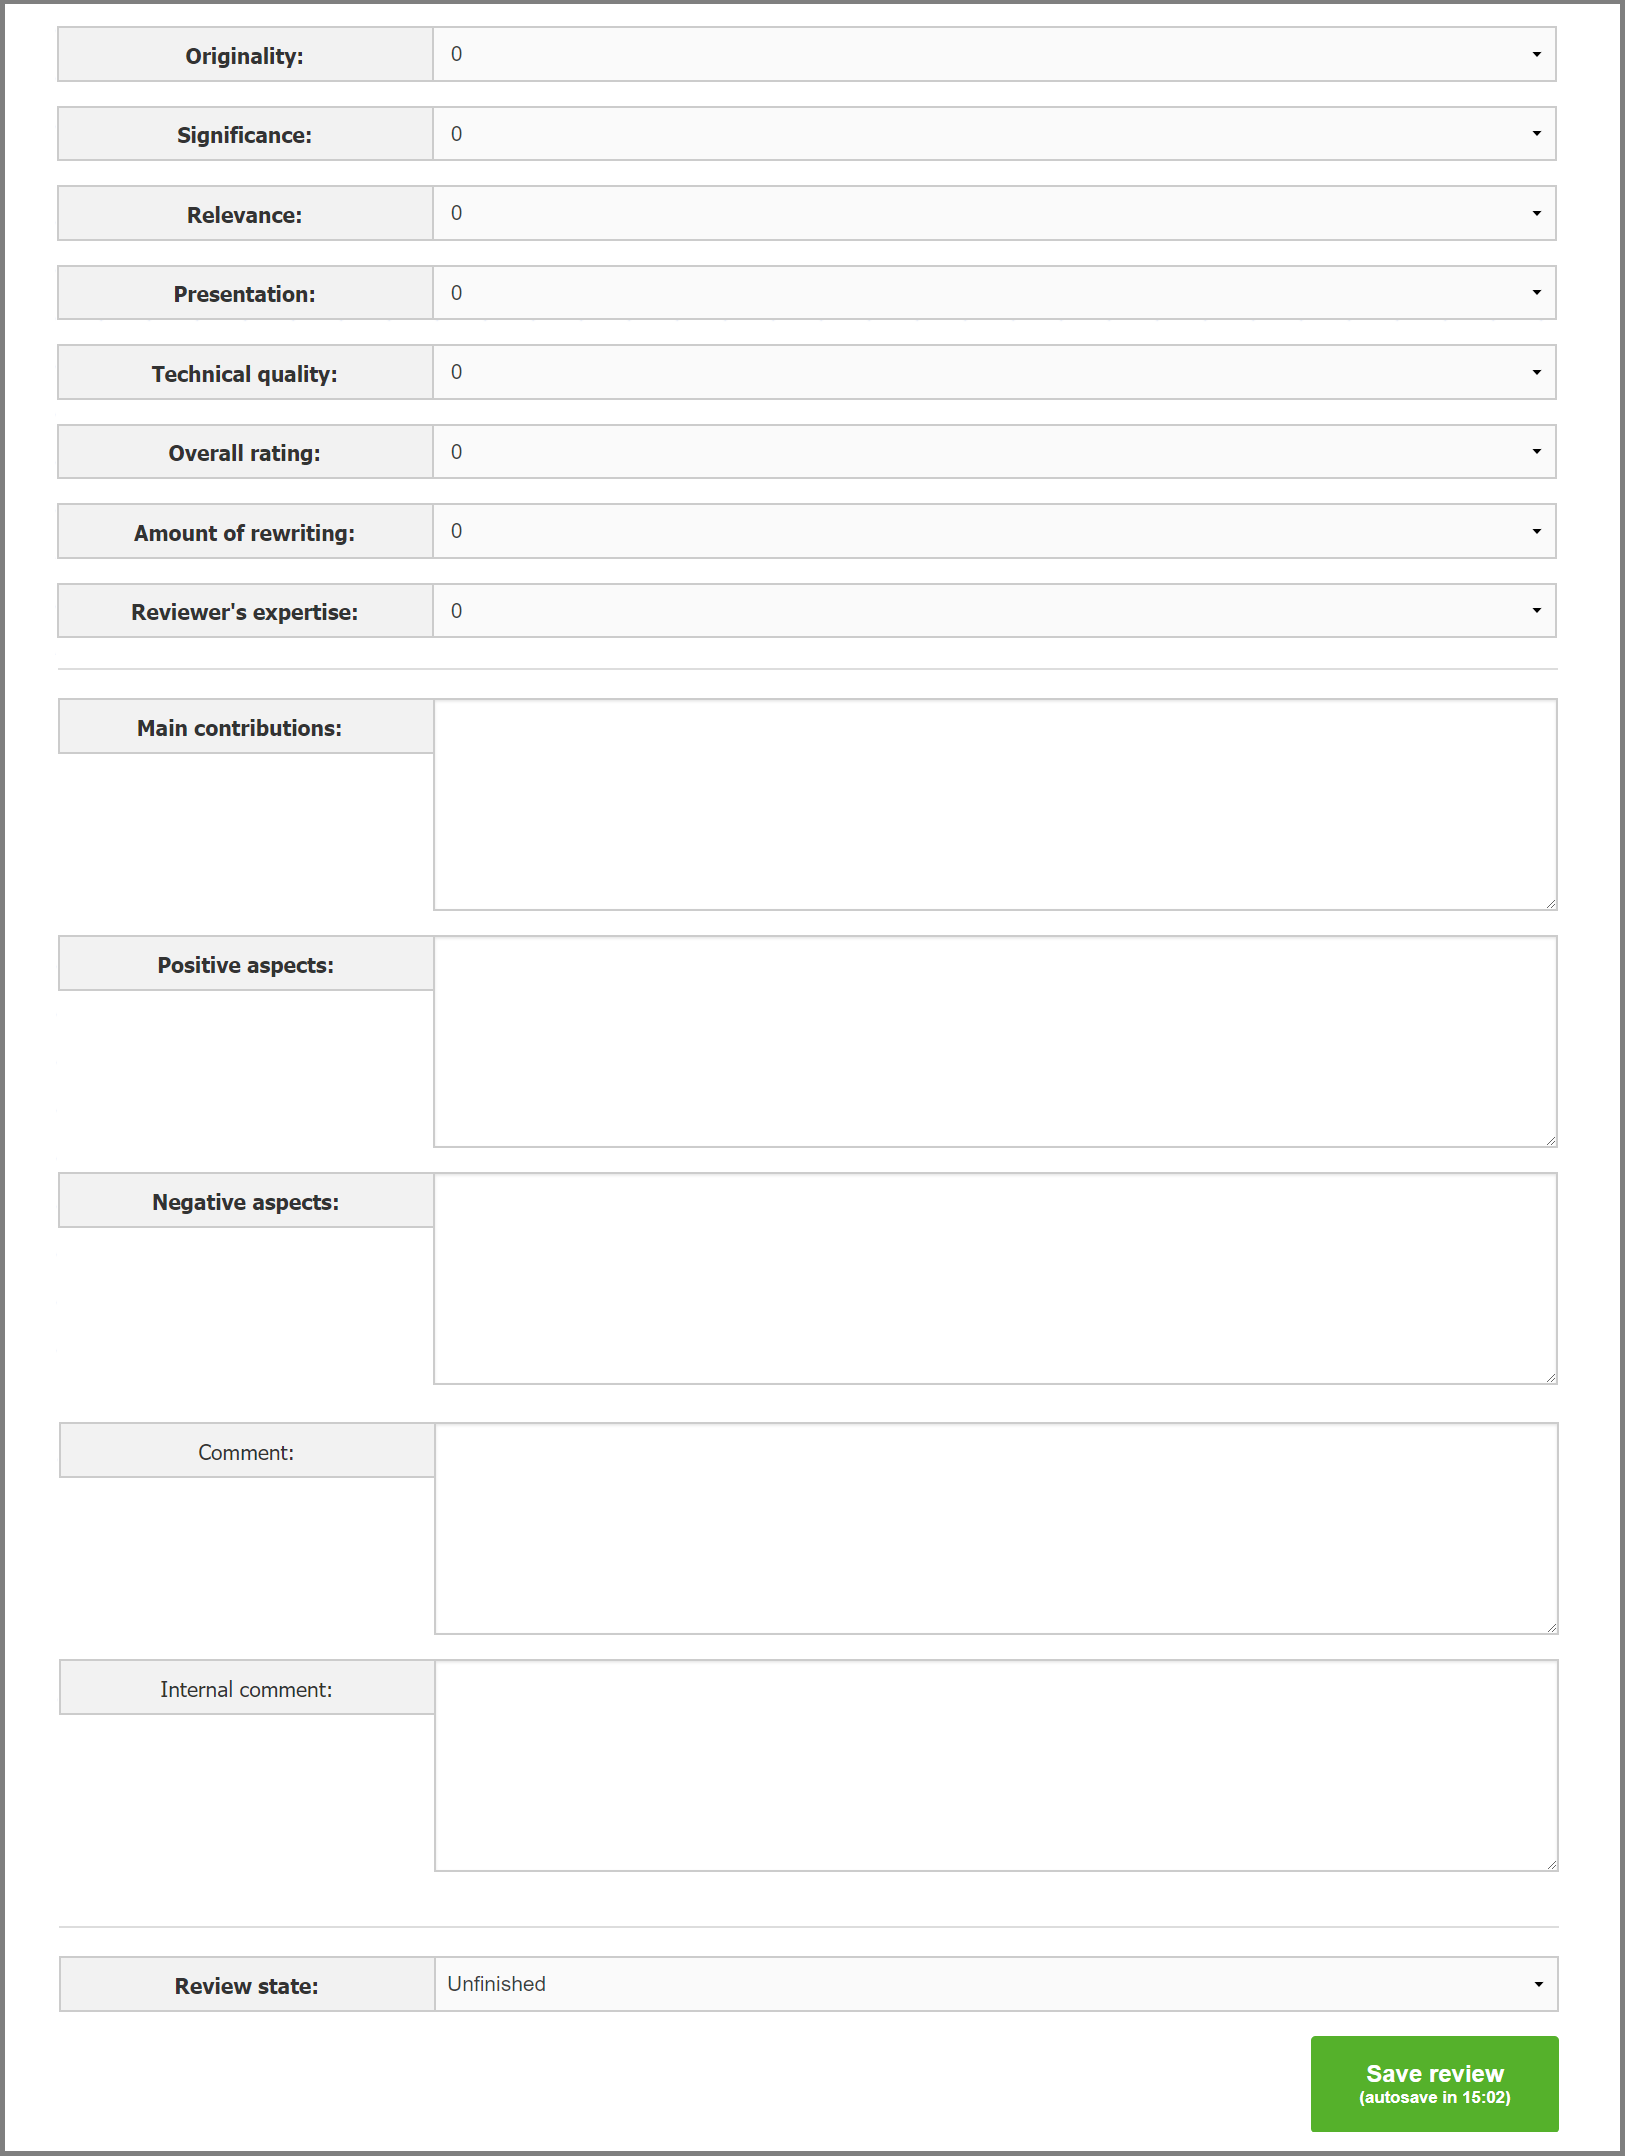
\includegraphics[width=15cm]{img/web_formular}
\caption{Webový formulář používaný pro hodnocení vědeckých příspěvků na portálu konference TSD}
\label{fig:web_formular}
\end{figure}

%SECTION
\section{Hlavní funkce modulu}
Vyvíjený modul musí být napsán stejným stylem jako je celý webový portál konferenčního systému TSD. Jelikož se na tomto portálu vyskytuje modul, který má stejnou funkcionalitu jako modul vyvíjený autorem bakalářské práce, tak je návrh funkcí jednodušší. Modul vyskytující se na portálu implementuje 3 důležité funkce, které zajišťují veškerou funkcionalitu i přes to, že pro zpracovávání PDF souborů je použit externí program \textit{PDFtk}. Po konzultaci s vedoucím práce bylo rozhodnuto, že se původní názvy funkcí zachovají a budou pouze změněny jejich parametry. Autorův modul bude tedy ve výsledku obsahovat, stejně jako starý modul, 3 důležité funkce doplněny o pomocné funkce a konstanty. Všechny hlavní funkce jsou popsány níže.  

%SUBSECTION
\subsection{Funkce pro generování}
Pro generování PDF souboru byla navržena 1 funkce. Tato funkce má za úkol nejdříve nastavit veškeré fonty a styly pro vzhled dokumentu, následně využít vhodný generátor PDF souborů, který vytvoří všechny části dokumentu (vypsané v kapitole \ref{sec:navrh_vzhledu}) a nabídne uživateli možnost stáhnout si výsledný hodnotící PDF soubor. Návrh hlavičky funkce viz \ref{lst:generate_function}.

\lstset{style=phpstyle}
\begin{lstlisting}[caption = {Návrh hlavičky funkce pro generování PDF souboru}, label = {lst:generate_function}, captionpos=b]
function generate_offline_review_form($rid, $reviewer_name, $sid, $submission_name, $submission_filename)
\end{lstlisting}
Popis vstupních parametrů funkce:
\begin{itemize}
	\item\textcolor{blue}{\textbf{\$rid}} -- ID hodnotícího příspěvku
	\item\textcolor{blue}{\textbf{\$reviewer\_name}} -- Celé jméno posuzovatele
	\item\textcolor{blue}{\textbf{\$sid}} -- ID vědeckého příspěvku
	\item\textcolor{blue}{\textbf{\$submission\_name}} -- Celý název vědeckého příspěvku
	\item\textcolor{blue}{\textbf{\$submission\_filename}} -- Celý název PDF souboru vědeckého příspěvku
\end{itemize}

%SUBSECTION
\subsection{Funkce pro zpracování}
Pro zpracování  PDF souboru byly navrženy 2 funkce, kdy první z nich má za úkol nahrát celý soubor do konferenčního souboru. Po nahrání souboru začne extrakce dat pomocí vhodných parserů a jejich zpracování. Následně se vše uloží do vhodných struktur a všechny extrahované hodnotící parametry se předají do následující funkce. Návrh hlavičky funkce viz \ref{lst:process_function}.

\begin{lstlisting}[caption = {Návrh hlavičky funkce pro extrakci dat}, label = {lst:process_function}, captionpos=b]
function process_offline_review_form($rid, $sid, $revform_filename)
\end{lstlisting}
Popis vstupních parametrů funkce:
\begin{itemize}
	\item\textcolor{blue}{\textbf{\$rid}} -- ID hodnotícího příspěvku
	\item\textcolor{blue}{\textbf{\$sid}} -- ID vědeckého příspěvku
	\item\textcolor{blue}{\textbf{\$revform\_filename}} -- Celý název PDF souboru hodnotícího příspěvku
\end{itemize}

Druhá funkce pro zpracování PDF souboru má za úkol uložit již extrahované hodnotící parametry do databáze konferenčního systému. Návrh hlavičky funkce viz \ref{lst:upload_function}.

\begin{lstlisting}[caption = {Návrh hlavičky funkce pro uložení dat do databáze}, label = {lst:upload_function}, captionpos=b]
function upload_to_DB_offline_review_form($rid, $values)
\end{lstlisting}
Popis vstupních parametrů funkce:
\begin{itemize}
	\item\textcolor{blue}{\textbf{\$rid}} -- ID hodnotícího příspěvku
	\item\textcolor{blue}{\textbf{\$values}} -- Seznam všech hodnotících parametrů 
\end{itemize}